With an overview of our activities’ dependencies and a clear understanding of our critical path and activity slack, we were ready for the planning of the project and establishing deadlines. 
When making our actual activity plan for the project, we chose to use a planning tool called a Gantt chart. This planning tool shows the activities on one axis with time on the other, which gives an immediate visual overview of the chronological order of activities. Since we had valuable knowledge about the dependencies of activities, we chose a variant of the Gantt chart, which also shows these.
Our Gantt chart can be seen below.  

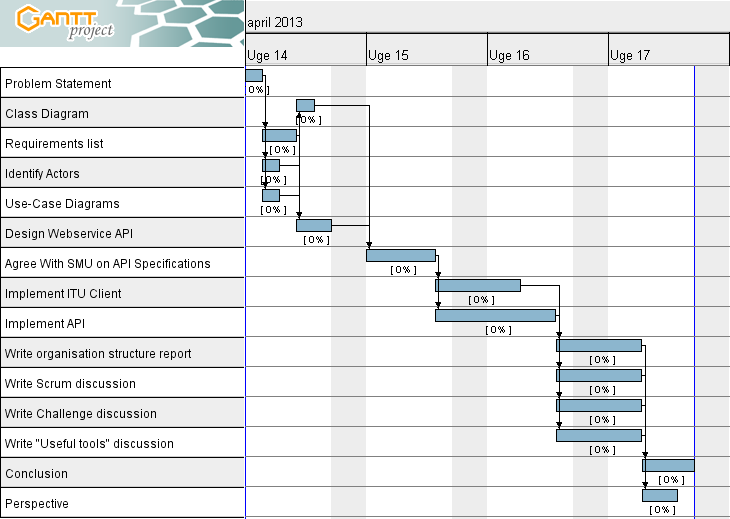
\includegraphics[scale=0.5]{./Empiri/Planning/img/gantt-chart.png}

%\textbf{Til analysefolk: 
%Burde vi evt. have lavet ressourceplaner? Dunno hvad det er..
%Also, bogen siger på side 132 at det er ”much better” ikke at bruge Gantt diagrammer med dependencies vist, fordi det bliver rodet.. De anbefaler et netværksdiagram i stedet, men det har vi jo ligesom OGSÅ lavet}
